\newif\ifpagetuning

\pagetuningtrue % trying to get page breaks in the best spots

\newif\ifnotcutting \notcuttingfalse % set if not cutting down to size


 \newif\ifpdfmadness

\ifx\pdfoutput\undefined
   \pdfmadnessfalse
\else
   \ifnum\pdfoutput=1
     \pdfmadnesstrue
   \else
     \pdfmadnessfalse
   \fi
\fi

\documentclass[preprint,nonatbib,blockstyle,nocopyrightspace,times]{sigplanconf}

\newcommand\txprobj[3][]{a#1_{#2_{j-1}#3_j}}
\newcommand\txprobjj[3][]{a#1_{#2_{j-1}#3_j}}
\newcommand\alignwidth{\ensuremath C} % number of columns in an alignment
\newcommand\pairedwith[1]{{\pi(#1)}}

\ifpagetuning
  \newcommand\tuningbox{\vbox}
\else
  \newcomming\tuningbox{\relax}
\fi

\newcommand\naive{na\"\i ve}
\usepackage{url}
\usepackage{amsmath}
\usepackage{array}
\usepackage{listings}
\usepackage{graphicx}
\lstset{
    tabsize = 2,
    basicstyle = \ttfamily,
    language = Haskell
    }    

\newcommand\figref[1]{Figure~\ref{#1}}
\newcommand\secref[1]{Section~\ref{sec:#1}}
\newcommand\seclabel[1]{\label{sec:#1}}

\usepackage{verbatim}

\newenvironment{smallverbatim}{\par\small\verbatim}{\endverbatim}
\newcommand\smallverbatiminput[1]{{\par\unskip\small\verbatiminput{#1}}}
\newcommand\smallfuzzverbatiminput[2]{{\par\unskip\small\hfuzz=#1 \verbatiminput{#2}}}

\renewcommand\ttdefault{aett}

  \long\def\remark#1{%
      \ifvmode
         \marginpar{\raggedright\hbadness=10000
         \parindent=8pt \parskip=2pt
         \def\baselinestretch{0.8}\tiny
         \itshape\noindent #1\par}%
      \else
          \unskip\raisebox{-3.5pt}{\rlap{$\scriptstyle\diamond$}}%
          \marginpar{\raggedright\hbadness=10000
         \parindent=8pt \parskip=2pt
         \def\baselinestretch{0.8}\tiny
         \itshape\noindent #1\par}%
      \fi}

\usepackage[authoryear]{natbib}
\bibpunct();A{},
\let\cite\citep
\let\citeyearnopar=\citeyear
\let\citeyear=\citeyearpar


\begin{document}


\conferenceinfo{ICFP '12}{September 9-15, Copenhagen.} 
\copyrightyear{2012} 
\copyrightdata{[to be supplied]} 

%\titlebanner{banner above paper title}        % These are ignored unless
\preprintfooter{Haskell in Computational Biology}   % 'preprint' option specified.

\title{Experience Report: Haskell in Computational Biology}
% \subtitle{Subtitle Text, if any}


\authorinfo{Noah M. Daniels \and Andrew Gallant \and Norman Ramsey}
           {Department of Computer Science, Tufts University}
           {{\rmfamily\{}ndaniels, agallant, nr{\rmfamily\}}@cs.tufts.edu}


\maketitle

%
% It can't hurt to remind everyone involved exactly what an Experience
% Report is.
%
%
\begin{abstract}
An Experience Report provides {evidence} that functional
programming really works, or it describes obstacles that prevent
functional programming from working.   
Here, we show that for computational biologists,
Haskell combines the flexibility and rapid prototyping of a scripting
language with performance comparable to~C++.
The~Haskell language and libraries provide powerful abstractions, 
but we couldn't always get them to work.
Despite some speed bumps around profiling, debugging, and the
uncertain status of any given package, we~found that Haskell's ecosystem
made it easy for us to develop new algorithms in computational
biology.
\end{abstract}

% \category{CR-number}{subcategory}{third-level}
% 
% \terms
% term1, term2
% 
% \keywords
% keyword1, keyword2

\section{Introduction}

Computational biologists write software that answers questions about 
sequences of nucleic acids (genomic data) or sequences of amino 
acids (proteomic data). 
For some software, considerations of performance are paramount; this
software is usually written in C~or~C++. 
For other software, considerations of convenience, readability, and
productivity are more important;
this software is usually written in a high-level
or domain-specific language like
Perl, Python, Ruby, SPSS, or~R.
In~this paper, we report on an attempt to replace both these families
of languages with Haskell: 
\begin{itemize}
\item
Although had to write a new implementation of a standard
algorithm, the cost was low, and the connection between code and
algorithm is unusually strong (\secref{viterbi}).
Our new Haskell code performs competitively with~C++,
and parallel performance was easy to achieve
(\secref{perf}). 
\item
Higher-order functions made it unusually easy to
implement and experiment with a family of related algorithms
(\secref{hofs}).
\item
The only significant impediment that Haskell presented to our
research was the difficulty of understanding and improving the
performance of Haskell programs (\secref{awkward-profiling}).
\item
We~used Haskell successfully even though we are computational
biologists with little background in functional programming.
Modifying our group's C++ code to try new research ideas has been
difficult;
trying new ideas in Haskell has been easy
(\secref{comparo}).
\item
The Haskell language is surrounded by a penumbra of libraries and tools that
promise powerful abstractions.
Some deliver very high leverage, but others are not ready for prime
time.
We~found the two families difficult to distinguish in advance (\secref{penumbra}).
\end{itemize}




\section{The biology}

Proteins are cellular machinery. They interact with one another and with other 
molecules to carry out the functions of living cells: metabolism, regulation, 
signalling, and so on.
A~protein's function is determined by its structure, 
and its structure is determined by the sequence of amino acids that
form the protein.
The amino-acid sequence is ultimately determined by a sequence of
nucleic acids in DNA, which we call a gene.
Given a genetic sequence, biologists wish to know the cellular
function of the protein that gene codes for.
The best known method of discovering such function is
to find other proteins of 
similar structure, which likely share similar function.
Proteins that share structure and function are expected to be
descended from a common ancestor---in biological terms, \emph{homologous}---and
thus
the problem of identifying proteins similar to a \textit{query sequence} is called 
\textit{homology detection}.




Computational biologists detect homologies by building 
algorithms which, given a {query sequence} of amino acids,
find known proteins of similar structure.
When the similar proteins are formed from amino-acid sequences that
are not too different from the query sequence, the homology can be
detected by
a family of algorithms called 
\textit{hidden Markov models}~\cite{Eddy:1998ut}.
But in real biological systems,
proteins with similar structure and function may be formed from significantly 
different amino-acid sequences, which are not close in edit distance.
Our~research contribution---a software tool called MRFy (pronounced
``Murphy'')---can detect homologies 
in amino-acid sequences that are only distantly related.
%
%We will explain an 
%algorithm for detecting reasonably similar sequences, and then move on to 
%explain MRFy, our novel approach for detecting more distantly related sequences 
%for proteins that share similar structure and function.
%

%
% I hope the new intro renders these two sentences unnecessary. ---NR
%
%
%%  
%%  To~enable you to understand our experience with Haskell,
%%  we~sketch not only the MRFy algorithm (\secref{mrfy})
%%  but also one of the older hidden-Markov algorithms (\secref{viterbi}),
%%  which is incorporated into~MRFy.


\section{The Software}



Homology-detection software is most often used in one of two ways:
to test a hypothesis about 
the function of a single, newly discovered protein, or 
to compare every protein in a genome against a library of known protein 
structures.
Either way, 
the software is \emph{trained}
on a group of proteins that share function and structure.
These proteins are identified by a biologist, who puts
their amino-acid sequences into a correspondence, also called an
\emph{alignment}. 
This alignment relates individual amino acids in a set of homologous proteins.
An~alignment may be represented as a matrix
in which each row corresponds to the amino-acid sequence of a protein,
and each column groups amino acids that play similar roles in
different proteins (Figure~\ref{alignment}).


An alignment may contain \emph{gaps}, which in 
\figref{alignment} are shown as dashes.
A~gap in row~2, column~$j$ indicates that as proteins evolved, either 
protein~2 lost its amino acid in position~$j$, or 
other proteins gained an amino acid in position~$j$.
If~column~$j$ contains few gaps, 
it~is considered a \emph{consensus column},
and the few proteins with gaps probably lost amino acids via
\emph{deletions}.
%%  \remark{NMD: Missing is the fact that all these models
%%  are directionless; they don't care whether something was gained or lost
%%  over time. But this doesn't matter.}
If~column~$j$ contains \emph{mostly} gaps, 
it~is considered a \emph{non-consensus column},
and the few proteins without gaps probably gained amino acids via
\emph{insertions}. 

Once a protein alignment is constructed, it~is used to train a
\emph{hidden Markov model}. 
A~hidden Markov model is a probabilistic finite-state machine which 
can assign a probability to any query sequence.
A~protein whose query sequence has a higher probability is more likely to %
be homologous to the proteins in the alignment.
We~write a query sequence as $x_1, \ldots, x_{\scriptscriptstyle N}$,
where each $x_i$~is 
an amino acid.
$N$~need not be the same as the number of columns in the alignment,
which we write~\alignwidth.


\begin{figure}
\ifpdfmadness
\centerline{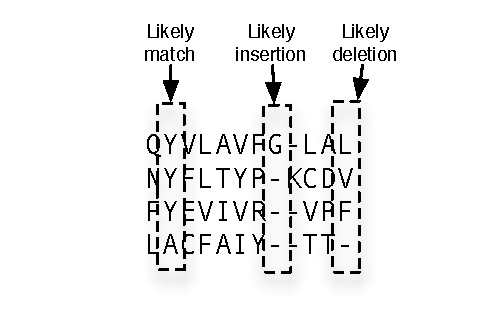
\includegraphics[width=6cm]{alignment.pdf}} 
\else
\centerline{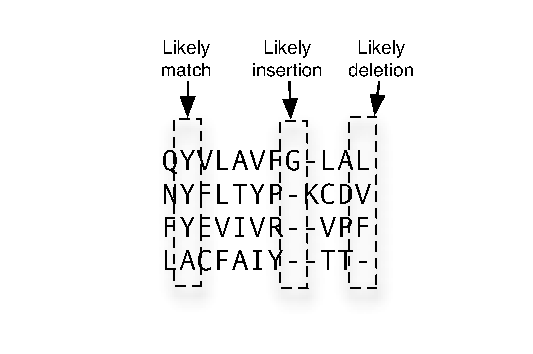
\includegraphics[width=6cm]{alignment.eps}} 
\fi

\caption{A~structural alignment of four proteins $(\alignwidth = 12)$}
\label{alignment} 
\end{figure}



A~hidden Markov model carries probabilities on some states and on all
state transitions.
Both the probabilities and the
the states are determined by the alignment:
\begin{itemize}
\item
For each column~$j$ of the alignment, the hidden Markov model has a
\emph{match state}~$M_j$.
The match state contains a table $e_{M_j}(x)$ which gives the
 probability that a homologous protein has amino acid~$x$ in
 column~$j$.
This probability is called an \emph{emission} probability.
\item
For each column~$j$ of the alignment, the hidden Markov model has a
\emph{deletion state}~$D_j$.
The deletion state determines the probability that the query sequence
has \emph{no} amino acid  in column~$j$, i.e., that it has a gap.
\item 
For each column~$j$ of the alignment, the hidden Markov model has an
\emph{insertion state}~$I_j$.
The insertion state contains a table $e_{I_j}(x)$ which gives the
probability that a homologous protein has gained amino acid~$x$ by
insertion at column~$j$.
\end{itemize}
The hidden Markov model also has distinguished \emph{begin} and \emph{end} states.
We~represent a state using an algebraic data type:
\begin{smallverbatim}
data HMMState = Mat | Ins | Del | Beg | End
\end{smallverbatim}


The particular hidden Markov model we use requires that every nonempty
sequence of insertions be followed by a match, and similarly for
deletions.
In~other words, insertions and deletions cannot be mixed without an
intervening match.
This restriction means that there are only seven possible transitions
into the states of any one column \cite{Eddy:1998ut}. 
\begin{itemize} 
\item
A~transition into a match state in
column~$j$ is more likely when column~$j$ is a consensus column.
Depending on the predecessor state, 
the probability of such a transition is 
$\txprobj M M$, $\txprobj I M$, or $\txprobj D M$.
\item
A~transition into a deletion state in
 column~$j$ is more likely when column~$j$ is a non-consensus column.
The probability of such a transition is 
$\txprobj M D$ or $\txprobj D D$.
\item
A~transition into an insertion state in
 column~$j$ is more likely when column~$j$ is a non-consensus column.
The probability of such a transition is 
$\txprobjj M I$ or $\txprobjj I I$.
\end{itemize}



\begin{figure} 
\ifpdfmadness
\centerline{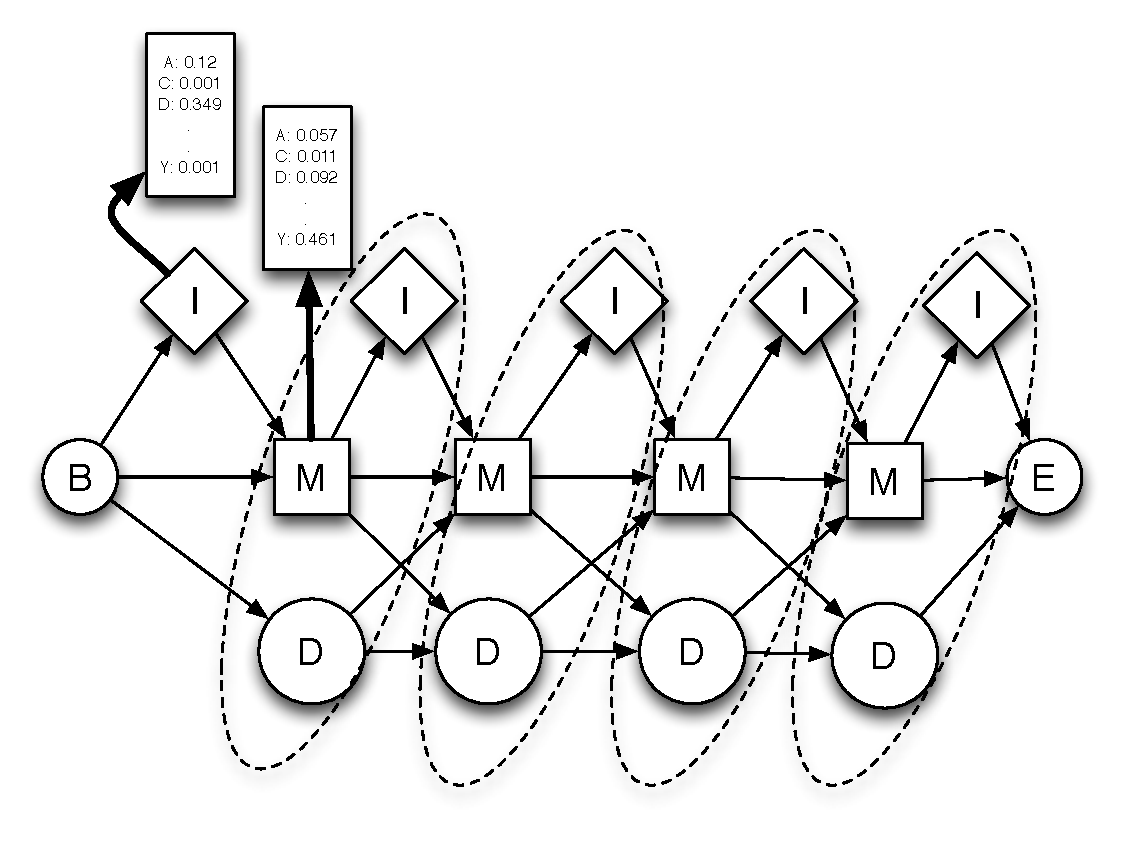
\includegraphics[width=8cm]{Plan7.pdf}} 
\else
\centerline{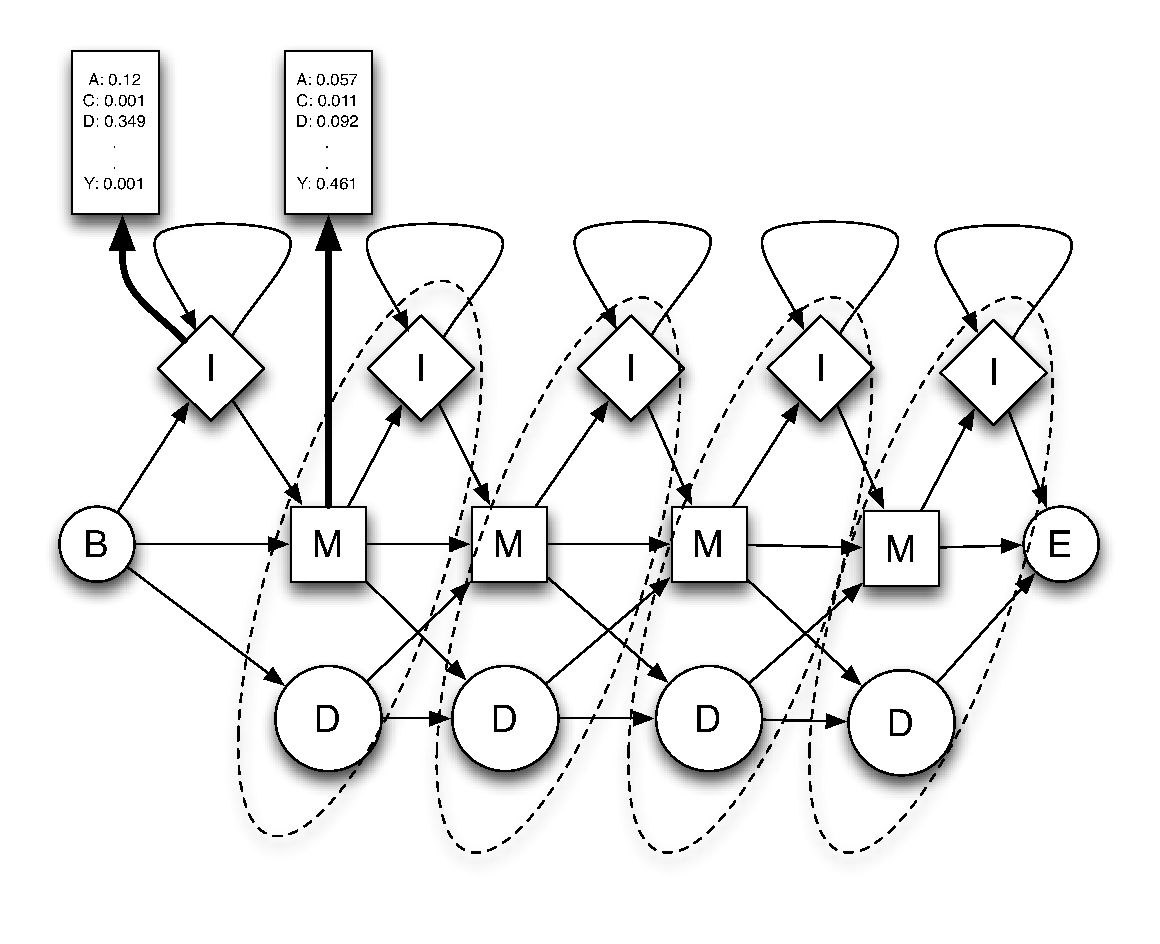
\includegraphics[width=8cm]{Plan7.eps}} 
\fi


This model
has begin and end states $B$~and~$E$,
as well as four
nodes, each containing 
an insertion state~$I$, 
a match state~$M$, and a
deletion state~$D$.

\caption{A hidden Markov model $(\alignwidth = 4)$}

\label{plan7} \end{figure}



\begin{figure*}
\newcommand\vsum[2]{#2&{}+{}& #1}

\def\goo{18pt}
\def\gum{14pt}
\[
\begin{array}{l@{}c@{}l}
V_{j}^{M}(i) &{}={}& \log\frac{e_{M_{j}}(x_{i})}{q_{x_{i}}} + \max \left\{
\begin{array}{l@{}c@{}l}
\vsum{V_{j-1}^{M}(i - 1)} {\log a_{M_{j-1}M_{j}}}\\
\vsum{V_{j-1}^{I}(i - 1)} {\log a_{I_{j-1}M_{j}}}\\
\vsum{V_{j-1}^{D}(i - 1)} {\log a_{D_{j-1}M_{j}}}\\
\end{array} \right.\\[\goo]
V_{j}^{I}(i) &=& \log\frac{e_{I_{j}}(x_{i})}{q_{x_{i}}} + \max \left\{
\begin{array}{l@{}c@{}l}
\vsum{V_{j}^{M}(i - 1)} {\log a_{M_{j}I_{j}}}\\
\vsum{V_{j}^{I}(i - 1)} {\log a_{I_{j}I_{j}}}\\
\end{array} \right.\\[\gum]
V_{j}^{D}(i) &=& \max \left\{
\begin{array}{l@{}c@{}l}
\vsum{V_{j-1}^{M}(i)} {\log a_{M_{j-1}D_{j}}}\\
\vsum{V_{j-1}^{D}(i)} {\log a_{D_{j-1}D_{j}}}\\
\end{array} \right.\\
\end{array}
\qquad
\begin{array}{l@{}c@{}l}
V_{j}^{\prime M}(i) &{}={}& e^{\prime}_{M_{j}}(x_{i}) + \min \left\{
\begin{array}{l@{}c@{}l}
\vsum{V_{j-1}^{\prime M}(i - 1)} {a^{\prime}_{M_{j-1}M_{j}}}\\
\vsum{V_{j-1}^{\prime I}(i - 1)} {a^{\prime}_{I_{j-1}M_{j}}}\\
\vsum{V_{j-1}^{\prime D}(i - 1)} {a^{\prime}_{D_{j-1}M_{j}}}\\
\end{array} \right.\\[\goo]
V_{j}^{\prime I}(i) &=& e^{\prime}_{I_{j}}(x_{i}) + \min \left\{
\begin{array}{l@{}c@{}l}
\vsum{V_{j}^{\prime M}(i - 1)} {a^{\prime}_{M_{j}I_{j}}}\\
\vsum{V_{j}^{\prime I}(i - 1)} {a^{\prime}_{I_{j}I_{j}}}\\
\end{array} \right.\\[\gum]
V_{j}^{\prime D}(i) &=& \min \left\{
\begin{array}{l@{}c@{}l}
\vsum{V_{j-1}^{\prime M}(i)} {a^{\prime}_{M_{j-1}D_{j}}}\\
\vsum{V_{j-1}^{\prime D}(i)} {a^{\prime}_{D_{j-1}D_{j}}}\\
\end{array} \right.\\[\gum]
\multicolumn3{l}{%
a'_{s} = - \log a_{s} 
\qquad
e^{\prime}_{s,x} = - \log\frac{e_{s,x}}{q_{x}}
\qquad
V_j^{\prime M}(i) = - V_j^{M}(i)
}
\\
\end{array}
\]

\caption{Viterbi's equations, in original and negated forms}
\label{viterbi}
\end{figure*}



\subsection{Computing probabilities using perspicuous Haskell}

\seclabel{viterbi}


Given a hidden Markov model, 
an~established software package called HMMER (pronounced ``hammer'') 
can compute the probability
that a new protein shares structure and
evolutionary history with the proteins used to train the model.
The computation finds the most likely path through the hidden Markov model.
To~make best use of floating-point arithmetic, the software computes
the \emph{logarithm} of the probability of each path, by summing
the logs of the 
probabilities on the states and edges of the path \cite{Viterbi:1967hq}.
The logarithm function is monotonic, so the path that maximizes the
log of the probability is the most likely path.

The computation is specified on the left-hand side of \figref{viterbi}.
A~probability $V_j^M(i)$ represents the probability of the most
likely path of the first~$i$ amino acids in the query sequence,
terminating with placement of amino acid $x_i$ in state~$M_j$.
Probabilities $V_j^D(i)$ and $V_j^D(i)$ are similar.
These
equations are very clearly explained by
\citet[Chapter~5]{Durbin:1998wz}


To~be able to use Haskell, we had to reimplement the standard
algorithm for solving Viterbi's equations.
Haskell made it possible for us to write code that looks like the
math,
which made the code easy to write and gives us confidence that it is
correct.
To~present some code,
we~begin with representations.

In~idiomatic Haskell, 
we might represent an individual amino acid~$x$
using a value of algebraic data type:
\begin{smallverbatim}
data Amino = Ala | Cys | Asp | Glu | Gly | ...
\end{smallverbatim}
But our primary goal was to get something working quickly,
and our hidden Markov models are stored using a
legacy file format that represents each amino acid as a small integer.
Our representation is therefore
\begin{smallverbatim}
type AA = Int -- amino acid using HMMER coding
\end{smallverbatim}
Either way, a query sequence is (and should be) an immutable vector of
amino acids.
%type QuerySeq = Vector AA
%\end{smallverbatim}

The log of a probability is just a number.
To distinguish a transition probability from other numbers, we wrap it in
a value constructor:
\begin{smallverbatim}
type LogProb = Double
data TProb   = TProb { logProbability :: LogProb }
\end{smallverbatim}
We group transition probabilities into 7-tuples.
Each tuple corresponds to a ``node'' in the hidden Markov model
(a~dashed oval in \figref{plan7}) and to a column of the original
alignment.
As~noted above, 
a match state may transition to any state in the successor node;
an insertion state may transition to itself or to its successor match
state;
and
a~deletion may transition to its successor match
state or deletion state.
\begin{smallverbatim}
data TProbs = 
     TProbs { m_m :: TProb, m_i :: TProb, m_d :: TProb
            , i_m :: TProb, i_i :: TProb
            , d_m :: TProb, d_d :: TProb }
\end{smallverbatim}
In~our code, we select from this 7-tuple using the \texttt{edge}
function:
\smallverbatiminput{edge}
In MRFy, the first two arguments to \texttt{edge} are known at compile
time, and we expect \texttt{edge} to be inlined.

The representation of a node includes the probabilities of transitions
into the states of that node, plus the tables
of emission probabilities for the match and insertion states.
\begin{smallverbatim}
type EProbs  = Vector LogProb
data HmmNode = HmmNode { transitions  :: TProbs
                       , matEmissions :: EProbs
                       , insEmissions :: EProbs
                       }
\end{smallverbatim}

In~Viterbi's equations,
the probability in each state is a function of the probabilities
in its predecessor states, 
and all probabilities can be computed by a classic dynamic-programming
algorithm.
This algorithm starts at the begin state,
computes probabilites in nodes $1$~through~$\alignwidth$ in
succession, and terminates at the end state.
One of us implemented this algorithm, storing the probabilities in an array.
The cost was
$O(|N|\times|\alignwidth|)$;
in~MRFy, $\alignwidth$~and~$N$ range from several hundred to a few
thousand.



%%  For 
%%  reasons including floating point underflow, the HMMER software (with which we 
%%  maintain file format compatibility) stores all probabilities in a trained HMM 
%%  file as negative natural logs.
%%  Thus, the Viterbi recurrence relations are 
%%  simplified from the form in \ref{viterbi_eqn} to that in \ref{viterbi_log_eqn}, 
%%  and because they are \textit{negative} logs, the problem transforms from 
%%  maximization to minimization.

Another of us was curious to try coding Viterbi's equations
directly as recursive functions.
Like the classic recursive Fibonacci function, Viterbi's functions,
when implemented \naive ly,
perform extraordinarily badly.
But just like the Fibonacci function, Viterbi's functions can be
\emph{memoized}.
To~show our code, we have to confess to a 
transformation of Viterbi's equations.
The~logarithms on the left of \figref{viterbi} are computed when the
hidden Markov model is constructed, and the resulting numbers are
stored in a file.
And~to~make this file more pleasant to read, the logarithms are
negated.
(The logarithm of a probability is typically negative, and negating
the logarithm eliminates hordes of minus signs.)
We~therefore implement a transformed version of Viterbi's equations,
shown on the right-hand side of \figref{viterbi}.
The transformed equations minimize the
negated log probability for each combination of node~$j$, amino
acid~$x_i$, and state $M_j$, $I_j$, or $D_j$.
A~negated log probability is called a~\emph{score}.

MRFy computes not only the minimum score but
also the path of states which produces that score.
Scores can be usefully paired with many types of values,
so we have defined a small abstraction:
\smallverbatiminput{vscore}
Think of a value of type \texttt{Scored~a} as a container holding
 an~``\texttt a'' with a score written on the side.
The \texttt{/+/} function adds to the score without touching the
 container.

\tuningbox{
We~also made \texttt{Scored} an instance of~\texttt{Ord} and of
\texttt{Functor}, so
\begin{smallverbatim}
fmap :: (a -> b) -> (Scored a -> Scored b)
\end{smallverbatim}
applies a function to what's inside the container, without touching
the score.
And containers are ordered by score alone, so applying
\texttt{minimum} to a list of scored things chooses the thing with the
smallest (and therefore best) score.
}

Given the \texttt{Scored} abstraction, we can easily implement
Viterbi's equations for a match state.
To~implement the equation at the top right of \figref{viterbi},
we~choose the best solution
from among the three predecessor states;
we~use~\texttt{/+/} to add transition and emission scores,
and we use \texttt{fmap} to add \texttt{Mat} to the list of states
encountered up to this point:
%%%%%%%%%%%%%%%%%%%%%%%%%%%%%%%%%%%%%%%%%%%%%%%%%%%%%%%%
\smallverbatiminput{vfix}
Functions \texttt{tProb} and \texttt{edge} combine to select the
appropriate transition score (one of the $a'$~values).
Function~\verb+vee''+ is the \emph{memoized} version of~\verb+vee'+,
so
the call to~\verb+vee''+ produces the same result as a recursive call
to~\verb+vee'+, but faster:
\smallverbatiminput{memo}
Functions \texttt{Memo.memo3} and \texttt{Memo.arrayRange} come from
Luke Palmer's
\path{Data.Memocombinators} package.
The value
\texttt{numNodes} represents~$\alignwidth$,
and \texttt{seqlen} represents~$N$.

Memoization makes \verb+vee'+ perform just as well as the classic
dynamic-programming code.
And~the call to \texttt{Memo.memo3} is the \emph{only} part of the code
devoted to improving performance.
By~contrast, standard implementations of the Viterbi algorithm, such as in HMMER,
spend much of their code 
managing dynamic-programming tables.
Haskell enabled us write simple, performant code with little effort.
%
Because the memoized version so faithfully resembles the equations in
\figref{viterbi}, we~retired the classic dynamic-programming version.



%%  
%%  
%%  In this, we were grateful for the resemblance 
%%  between the mathematical description of the algorithm and the top-down 
%%  dynamic-programming approach in Haskell, which resulted in perspicuous code.
%%  
%%  


\subsection{Exploring new algorithms using higher-order functions}

\seclabel{hofs}
\seclabel{mrfy}

Our implementations of hidden Markov models and Viterbi's algorithm
duplicate existing functionality.
In~MRFy, they are used to implement new functionality.

A hidden Markov model uses local information about
amino-acid sequences.
But when a real protein folds in three dimensions, 
groups of amino acids 
that are far away in the one-dimensional sequence can be
adjacent in three-dimensional space.
We~are studying adjacent groups called \emph{beta strands}, which
can become hydrogen-bonded to each other,
and are effectively ``stuck together.''

A~mutation in a paired beta strand may break the pairing, in which
 case the mutated protein will not fold properly and is unlikely to
 survive natural selection.
But a mutation in a paired beta strand \emph{can} survive if it is
 accompanied by a \emph{compensatory} mutation in the strand with which it is
 paired. 
The probability of finding amino acid~$x_i$ in column~$j$ of an alignment may
 therefore depend on the amino acid in the paired column
 $\pairedwith j$.
This nonlocal interaction changes
Viterbi's equations:
each term $V_{j}^{\prime M}(i)$ becomes
$$W_{j}^{M}(i) = V_{j}^{\prime M}(i) - \log P(x_{i} \mid x_{\pairedwith j}).$$
The distance between columns~$j$ and $\pairedwith j$ can be as small
 as a few columns or as large as a few hundreds of columns.


The approach currently taken in computational biology
is~to model each pair of beta strands not with two hidden Markov
models, 
but with a pair of sequences of match states.
Each of the subsequences \emph{between} paired beta strands is then
modeled with an ordinary hidden Markov model.
The~combined model, an~example of which is shown in \figref{mrf}, is called a
\textit{Markov random field}. 
Because of nonlocal interactions between paired beta strands, 
the likelihood-maximization problem for a Markov random field does not
 exhibit optimal substructure, and dynamic
 programming cannot solve it quickly \cite{Menke:2010ti,Daniels:2012}.
MRFy explores new methods of \emph{approximating}
maximum likelihood.


\begin{figure}
\ifpdfmadness
\centerline{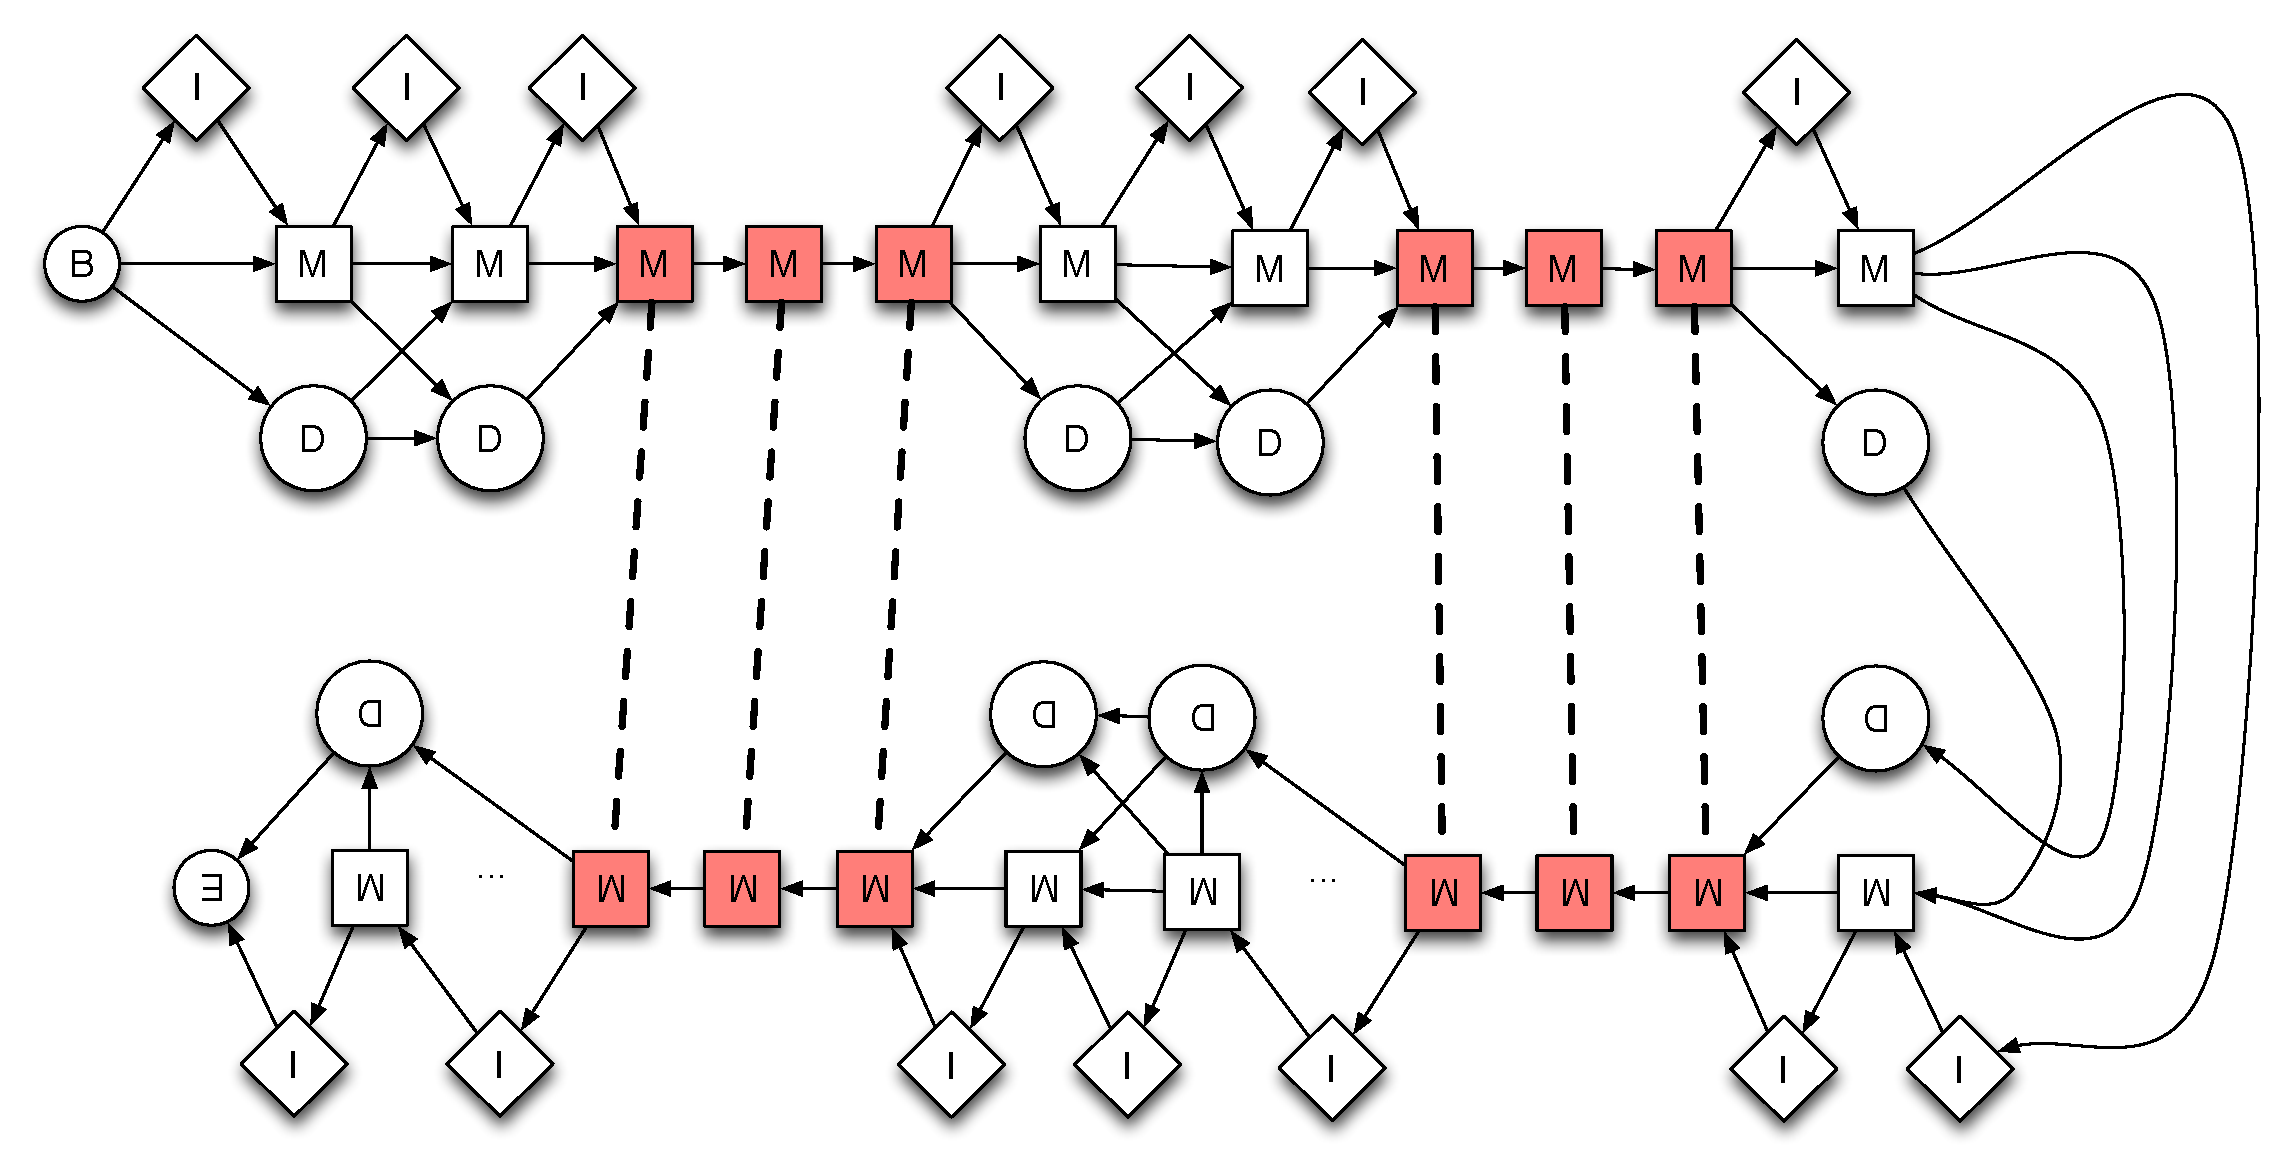
\includegraphics[width=8cm]{mrf_interleave_diagram.pdf}} 
\else
\centerline{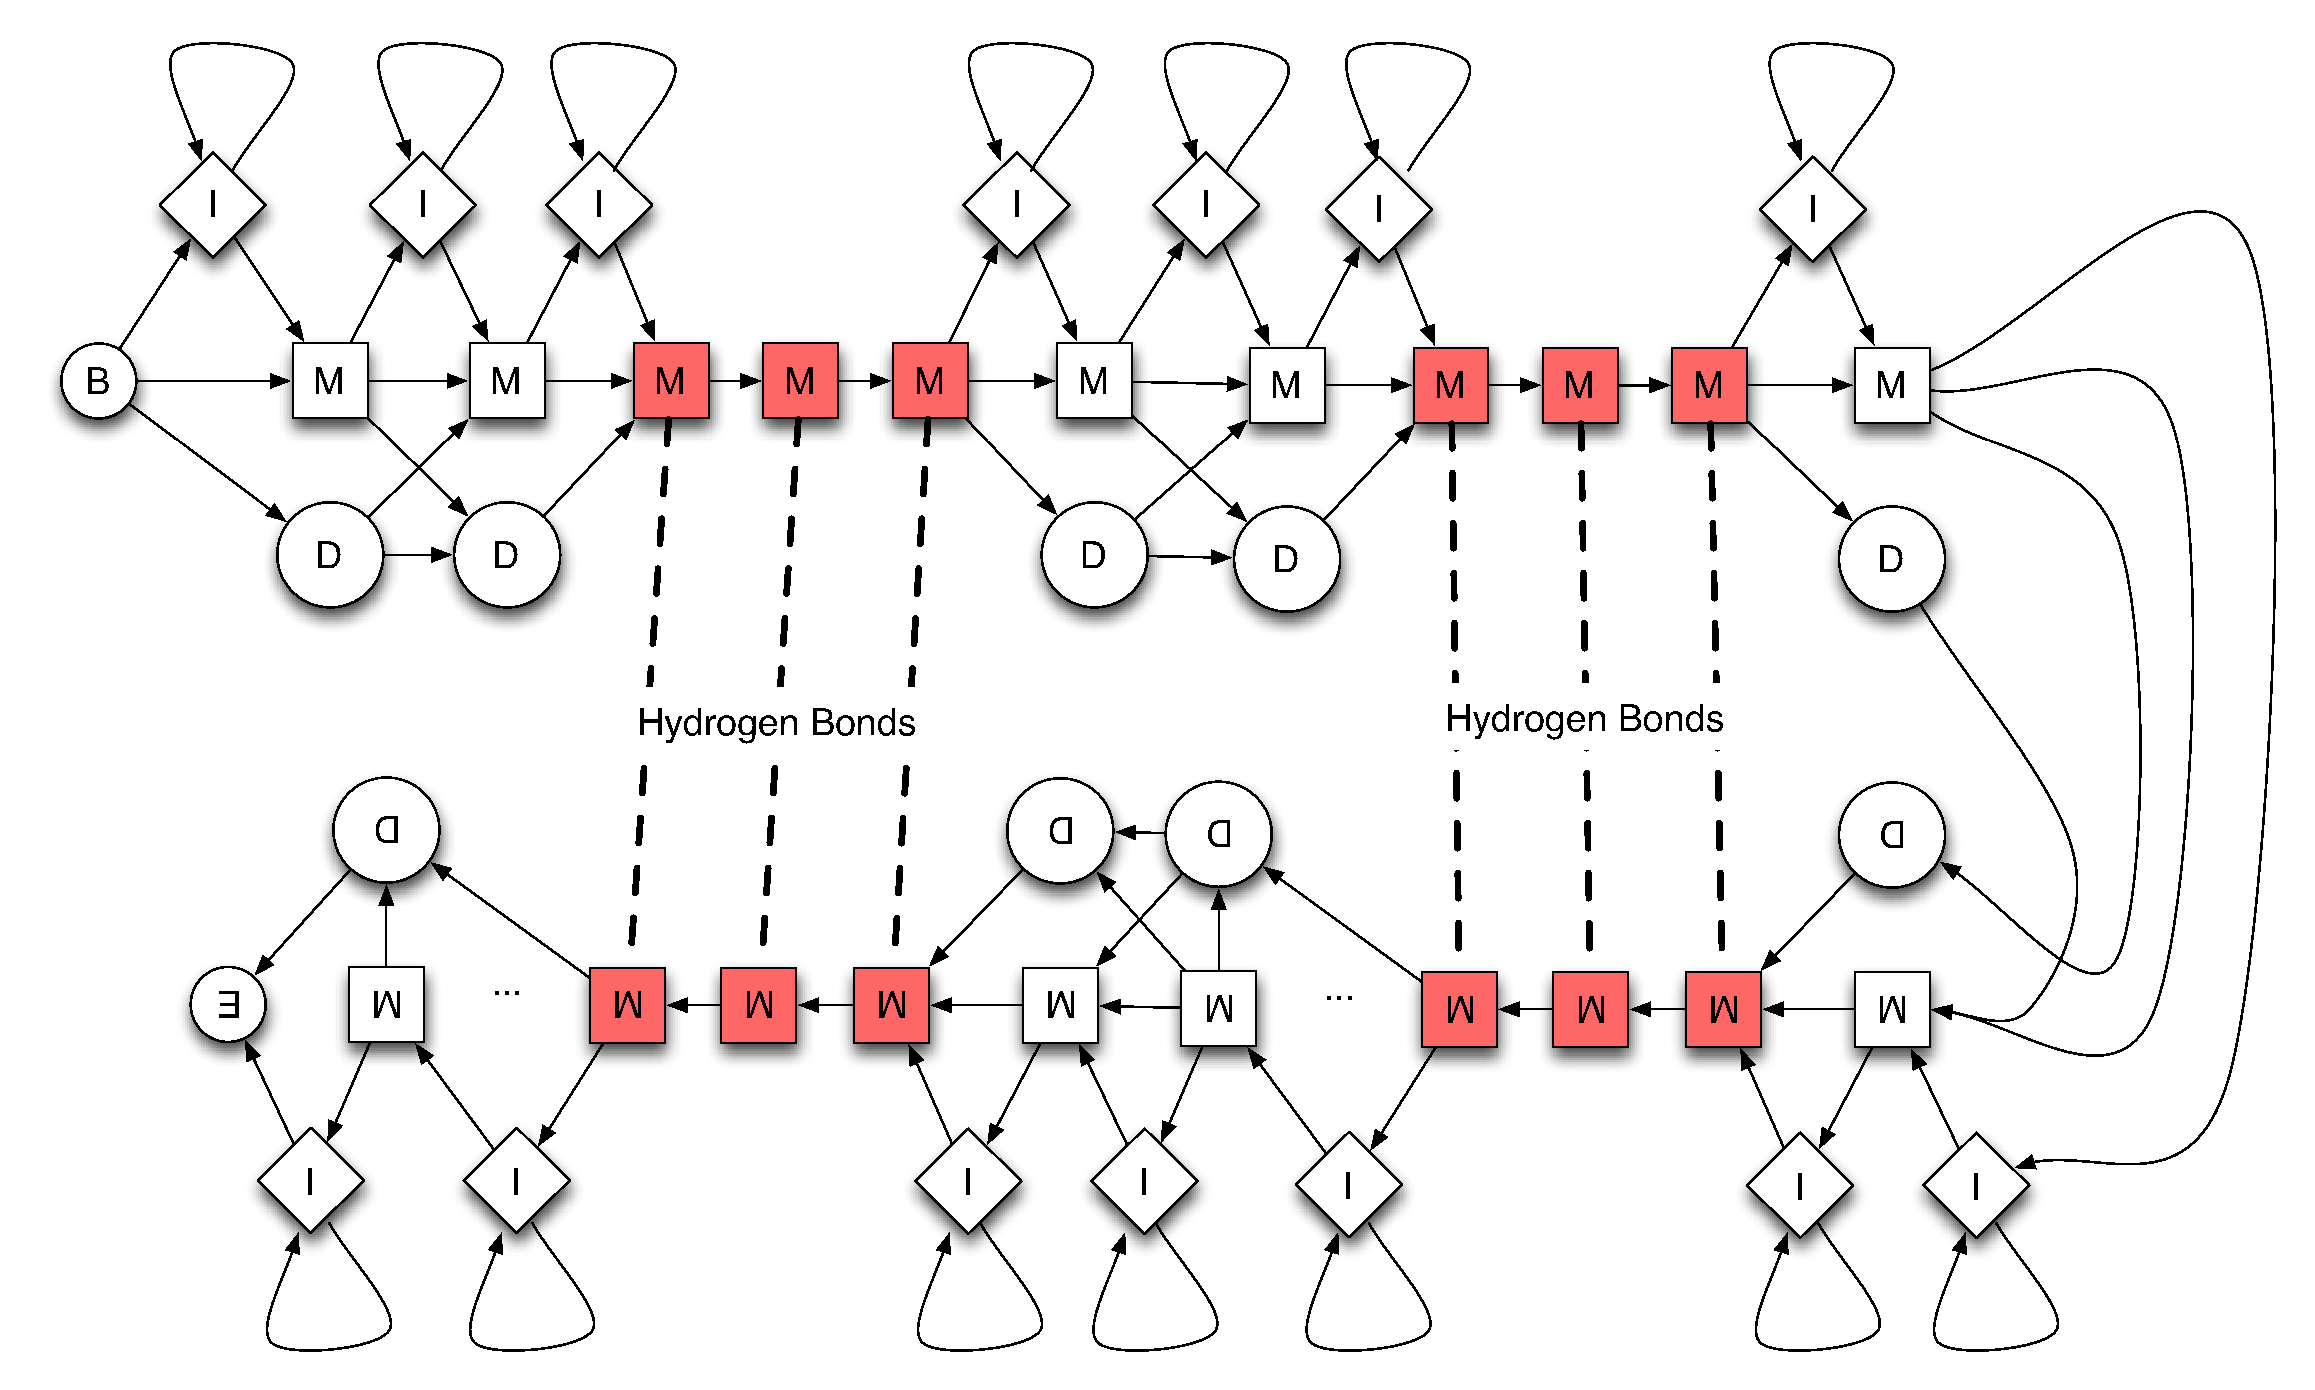
\includegraphics[width=8cm]{mrf_interleave_diagram.eps}} 
\fi
In this Markov random field,
each shaded node represents a beta-strand position.
Nodes connected by dashed edges are hydrogen-bonded.

\caption{A Markov random field with two beta-stand pairs}
\label{mrf} 
\end{figure}



MRFy treats the beta 
strands, which are built into the model,
 as ``beads'' which can be slid along the query sequence.
A~set of positions of beta strands is called
 a \emph{placement}.
A~placement's probability is computed
based on observed frequencies of paired amino acids in 
hydrogen-bonded beta strands~\cite{Cowen:2002p588}.
Given a placement, the maximum likelihood of any subsequence that appears
\emph{between} two beta strands can be computed exactly and
efficiently using Viterbi's algorithm.
(The result of the exact computation is a probability that is
\emph{conditioned} on the placement.)

MRFy searches for placements stochastically,
trying to minimize scores.
We~are exploring several stochastic algorithms: random-mutation hill
climbing, simulated  
annealing, multistart simulated annealing, and a genetic algorithm.
Our~exploration relies on higher-order functions.

MRFy's search computes a sequence of \emph{generations}.
A~generation is a collection of scored {placements}.
We~pass the
search function a \texttt{Scorer}, which runs Viterbi's algorithm.
\smallverbatiminput{scoredecl}
A~search heuristic is characterized by four functions, which are
bundled into a record called \texttt{SearchStrategy}.
\smallfuzzverbatiminput{2.3pt}{strategy}
In this record,
\begin{itemize}
\item
Function \texttt{gen0} produces the first generation of placements.
\item
Function \texttt{nextGen} produces a new generation of placements from
an existing generation.
Because scoring a placement is expensive, 
and some placements may persist from the old generation to the new
generation, \texttt{nextGen} works with \emph{scored} placements, not
bare placements.
\item
A~new generation produced by \texttt{nextGen} may be no better
than the generation it replaces.
When it is first produced, the new generation is ``on trial.''
The \texttt{accept} function decides whether to keep a new generation
or to try \texttt{nextGen} again with a different seed.
The \texttt{accept} function considers a list of type
\texttt{[Scored~Age]}.
At~the head of this list is the score of the best
placement of the trial generation, together with the \texttt{Age} of the trial
generation, which is the total number of generations tried.
The remaining elements of the list hold the history of scores and ages for
previously \emph{accepted} generations.
(The list omits generations that didn't survive the \texttt{accept} trial.)
For convenience, the \texttt{accept} function also receives
the \texttt{Age} of the trial generation.
\item
Finally, the \texttt{quit} function decides when to stop the search.
It~too considers the list of accepted generations and the age of the current
generation. 
\end{itemize}
This interface provides ample leeway for experiments.
For~example, random-mutation hill climbing accepts only generations
with better scores than their predecessors,
while simulated annealing may accept a generation with a worse score.
A~genetic algorithm uses \texttt{nextGen} to
combine placements from the previous generation, while
random-mutation
hill climbing simply permutes a placement into a new one.
The \texttt{quit} interface makes it easy
to implement such termination criteria as a fixed number of generations
or a limit of going $k$~generations without achieving more than $E$
improvement in score. 

\seclabel{search}

We hope you find the search simple and straightforward:
\smallfuzzverbatiminput{11pt}{search}


We found it easy to write several stochastic search heuristics thanks to
this framework.
We first implemented random-mutation hill climbing in one day and roughly
fifty lines of code.
We next implemented simulated annealing, and thanks to Haskell's module system,
we imported the \texttt{nextGen}, \texttt{gen0}, and \texttt{quit} functions
from the random-mutation hill climbing module.
Indeed, we had only to write a new \texttt{accept} function, comprising only ten
lines of code and half an hour of our time.
We then implemented a genetic algorithm approach; this was still able to import
existing \texttt{gen0} and \texttt{quit} functions, and its \texttt{accept}
function was only a few lines of code.
Understandably, though, the complexities of representing ``crossover'' of parent
placements required forty lines of code and much of a day of thought.

\subsection{Performance}

\seclabel{perf}

In MRFy, the \texttt{score} function calls \texttt{viterbi} several
 times
for each placement in each search generation.
Calls on query sequences between beta strands are independent,
as are calls on different placements.
We~found them easy to parallelize
using
\texttt{Control.Parallel},
simply substituting
\texttt{parmap rseq} for \texttt{map}.
Even when there is just one placement per generation,
MRFy can keep six cores busy,
and when our search algorithm uses multiple placements per generation,
it~can use all forty-eight cores on a compute server.


In~\secref{viterbi} above, the example case for the \texttt{viterbi}
function computes not just a score but also an optimal path.
MRFy's \texttt{search} function, in \secref{search}, uses only the
score.
Even though Haskell evaluation is lazy, the \texttt{viterbi} function
is still allocating thunks.
We~tried cloning and modifying the \texttt{viterbi} code to compute
only a score, with no path, and this change improved 
run-time performance by nearly 50\%.
But when \texttt{search} finally decides on a placement, we need a
version of \texttt{viterbi} that \emph{does} compute path, so we can
extract the optimal parse for that placement.

How could we keep the performance improvement without having to
maintain two versions of \texttt{viterbi}?
In~Lisp or Ruby we would have used macros or metaprogramming,
but we were not confident of our ability to metaprogram a solution
using Template Haskell.
Instead, we replaced the primitive cons in \texttt{viterbi} with a
call to a function of the same type, which we passed~in.
Passing the primitive~``\texttt{:}'' gives us a path,
and passing \verb+\_ _ -> []+ gives us the same
speedup as the cloned and modified~code.
But~although
this trick is simple and easy to implement, 
we~have an uneasy feeling that it may work only because of undocumented
properties of GHC's inliner, which may be subject to change without
notice. 

\subsection{Awkward Haskell}

\seclabel{awkward-profiling}

In two major areas, our lack of skills or knowledge resulted in ugly
Haskell.
The first is profiling.
GHC's profiling is based on cost centers \cite{sansom-pj},
and although GHC 
will happily add cost centers to top-level 
functions, much of our code is in nested functions.
We~know of no better technique than to add cost-center annotations to
each guard clause and nested function,
but these annotations made our code so ugly that we felt compelled to
remove them as soon as possible.
And without the annotations, we found GHC's call-site and allocation
profiles did not provide enough information to be useful.
We~miss valgrind, whose callgrind profiler gives us enough information
without \emph{any} annotations in the source.

Our other ugly code came from  attempts to debug
run-time errors.
MRFy uses a Markov random field which is represented in a legacy file
format that uses a poorly documented representation---when beta
strands overlap and are doubly paired, the invariants of the
representation are not clear.
Dealing with this representation is difficult no matter what
programming language is used, and faults are to be expected.
Using GHC, we had a hard time diagnosing run-time errors.
Extensive use of 
\texttt{trace} 
littered our code,
even when moved from our main code to wrapper functions.
We~weren't aware of the backtrace feature of GHC's profiler,
and even after we discovered that feature, the results weren't good enough.
Specifically, because the backtrace feature required profiling mode,
it could only be used in very small test cases that didn't always trigger
run-time errors, and one of us was unable to overcome difficulties in building
various libraries in profiling mode.
In~August 2011, 
Lennart Augustsson said that the biggest advantage of Strict
Haskell is getting a stack trace on error,
and Simon Marlow said that he may have figured out how to track call
stacks properly in a lazy functional language.
We~can't wait.

 
 
\section{Our previous experience compared}
\seclabel{comparo}

When performance has mattered, the members of our group, like other
computational biologists, have used~C++.
We~compare our experience with three tools:
\begin{itemize}
\item
Matt~\cite{Menke:2008wu} is used to create alignments like that shown
in \figref{alignment}.
It~comprises about 12,000 lines of~C++.
The only external tool or library it uses is \texttt{zlib}.
Its initial development took two years.
\item
SMURF
\cite{Menke:2010ti} is used to detect homologous proteins in the presence
of paired beta strands.
It~comprises about 9,000 lines of~C++, of which about 1,000~lines are
shared with~Matt.
It~uses no external tools or libraries.
Its initial development took a year and a half.
\item
MRFy is used to detect homologous proteins in the presence of paired
beta strands.
It~comprises about 1,200 lines of~Haskell
It~uses several external tools and libraries, of which the most
notable are PADS-Haskell, the \path{Data.MemoCombinators} library,
the BioHaskell bioinformatics library, and the \path{Data.Vector} library.
Its initial development took about three months.
\remark{Others were mostly full-time work, but no need to distinguish.}
\end{itemize}
Like much research software, all three of these tools were written
 in~haste.
We~have experience modifying the older tools.



We~modified Matt to use information about sequences as well as structure.
The modification added 2,000 lines of code, and it calls
external sequence aligners that we did not write.
We~thought the modification would take three months, 
but it took most of a~year.
Matt uses such
data structures such as mutable oct-trees, vectors, and arrays.
It~uses clever pointer arithmetic.
The mutable data structures were difficult to 
repurpose, and the pointer arithmetic was too clever for its own good: 
nearly every change resulted in new segfaults.

We~had hoped to extend Matt further, with support for partial alignments,
which we~expected to require only 
a cosmetic manipulation of the 
output, but
this feature wound up
 requiring deep information about some data structures,
and we had to give~up.
We~believe we could write an equivalent tool in~Haskell,
with most of Matt's performance, in at most nine months.

Our most painful experience was adding ``simulated evolution''
to~SMURF \cite{Daniels:2012}. 
Although simulated evolution represents a relatively minor
enhancement,
just understanding the existing code took several months.

We~built MRFy quickly, and we expect that
higher-order functions will MRFy easy to extend.
Each new addition to MRFy's stochastic search has taken at most a day
to implement.

%
% An Experience Report is about what you actually did, not what you
% wish to do :-)
%
%%  There are two major research ideas we wish to add to MRFy eventually, one of which
%%  \remark{how much should I say about profiles and alpha helices? ---NMD}
%%  involves looking at another type of nonlocal dependency (\textit{alpha
%%  helices} in contrast 
%%  to the current beta strands).
%%  We expect that thanks to algebraic data types and typeclasses, these
%%  enhancements will be at 
%%  most a few weeks of work; we do not believe these enhancements would
%%  even be feasible in SMURF. 
%%  Indeed, Daniels tried to add another of these enhancements to SMURF
%%  two years ago and gave up due 
%%  to the difficulty of the implementation.
%%  \remark{The above needs a lot of revision. It is a shitty first
%%  draft of a /P/. ---NMD} 

On the protein structures for which it was originally designed, SMURF can 
compute the parse of a query sequence to a MRF based on those structures in 
less than 10 seconds on a typical workstation.
However, on somewhat more 
complex protein structures, SMURF may take two to three minutes on the same 
hardware. 
On the most complex protein structures, SMURF exhausts all memory on 
any system we have available, and must be killed. 
In contrast, MRFy's runtime 
for any of these protein structures is typically less than 30 seconds. 
This 
meets the performance goals we had, and means that MRFy is fast enough to scale 
to whole-genome scans.



Haskell encourages hasty programmers to slow down.
We~have to get the types right,
which makes it hard to write very large functions.
To~get the code to typecheck, we~have to write type signatures, which
also serve as documentation.
And once the types are accepted by the compiler,
it~is not much more work to write contracts for important functions.
MRFy is still hasty work.
Many types could be simplified;
we're~sure we've missed opportunities for abstraction;
and we know that MRFy's decomposition into modules could be improved.
But despite being hasty programmers, we produced code 
that is easy to understand and easy to extend.
Our hastily written Haskell beats
our hastily written Ruby and~C++.



Looking beyond our research group to computational biology more
broadly, our experience with other software is better.
Little of it is written in functional languages, 
but much of the software shared by the community is excellent.
MRFy's training component was derived from that of~HMMER,
and
working with HMMER 
codebase was pleasant;
data structures and their
mutators are well documented. 
There is a 
BioHaskell library, part of which we use,
but it is not nearly as 
complete as BioPython or BioRuby, which are heavily used in the community.
We hope that tools for computational biology in
Haskell continue to mature. 

\section{What can you learn from our experience?}

If~you are a computational biologist, 
you can be productive in Haskell without extensive
experience.
Two~of us (Daniels and Gallant) are graduate students.
Daniels has taken a graduate seminar in functional programming, which
included some Haskell;
Gallant has taken a programming-languages course which included
significant functional programming but no Haskell.
Ramsey is a professor who has used Haskell and other functional
languages for several medium-sized projects,
but his contribution was limited to minor ranting and refactoring.


\subsection{Barriers}

In~\secref{awkward-profiling} above, we~mention the awkwardness of the
cost-center annotations required for profiling.
But~we also found it difficult just to get the profiler working.
In~particular, profiling requires that all installed libraries be recompiled
with profiling support.
We~were not able to achieve such recompilations consistently.


We~faced another barrier in testing.
One of us (Ramsey) kept ranting that we should test our code using 
QuickCheck \cite{claessen:quickcheck},
but we could never figure out~how.
We~were stumped by two problems:
how to break down a complex module into parts that can usefully be
unit tested,
and how to implement QuickCheck generators for representations of complex
data like beta-strand placements.
We~know that QuickCheck is a powerful and proven tool,
yet we were not smart enough to figure out how to use~it.

Like other functional programmers, we~have found that often enough,
once we have the types right, the code is right.
But~much of our work involves computing with arrays and array indices,
and in that domain, types don't help much.
And we haven't been able to identify any systematic way of debugging
run-time errors in Haskell programs.
GHC's profiler can provide stack traces, but we~found this information
difficult to discover, and as noted above,
there are barriers to profiling.
We're~aware that debugging lazy functional programs has been a topic
of some research,\remark{Do we cite Hood, Hat, or Freya?}
but one of the biggest barriers we encountered to using Haskell is
that we have had to abandon our old approaches to debugging,
and we~see no clear path to follow.


\subsection{Information that will help you succeed}

If~you want to use Haskell in your research, we~believe that you must
have enough experience with functional programming that you can build
\emph{all} the code you need, not only the code that is easy to write
in a functional language.
Implementing Viterbi's equations in Haskell was pure joy.
Writing an iterative search in purely functional style was not
difficult.
When we had to transform data in the HMMER file format, \emph{without}
using mutable state the way the C++ code does, we~struggled.

\seclabel{penumbra}

You~also need to know that while the Haskell community offers many
enticing tools, libraries, and packages,
not all of them are worth using.
Some are not ready for prime time, and some were once great but are
no~longer maintained.
The great packages, like \texttt{Data.Memocombinators} and Parallel
Strategies, are truly great.
But~for amateurs, it's not always easy to tell them from the wannabes
and the has-beens.

Most of the software we used came from Hackage, which is the Haskell
community's software repository.
We~sometimes found it hard to tell
if a particular Hackage package was right for us.
In particular, as beginning 
functional programmers, we~found some documentation inaccessible.
The documentation that we found most accessible typically contained
examples showing how to use a particular tool or library.
\remark{So what's our message here? What are we telling people to
think or do differently? ---NR}


As~in any endeavor, it's helpful to have access to experts.
We~would have been better off if our in-house expert had been an
enthusiastic student and not a busy professor.
But we have been surprised and pleased by the help available from
faraway experts on Stack Overflow and on Haskell mailing lists.
Although a local expert makes things easier, one is not
 absolutely necessary.


\section{Conclusion}

A~little knowledge of and a lot of love for functional programming was
enough for us to carry out a successful research project in a language
that computational biologists seldom use.
If~you \emph{want} to use Haskell---or one of your graduate students
wants to use Haskell---you can
succeed. 




% - No obvious body of knowledge on code improvement. 
%  

 

\ifnotcutting
\acks

We thank Lenore Cowen, Kathleen Fisher, Benjamin Hescott, Bradford
Larsen, and Nathan Ricci. 
\fi


\bibliographystyle{plainnat}

% The bibliography should be embedded for final submission.

\bibliography{mrfy_experience_report}



\vfill

\begingroup
\parfillskip=0pt
\advance\leftskip by 0pt plus 30em
\emph{You can live to surf the Haskell wave, but~if you slide off the crest, you
drown.}
\par
\endgroup


\break


\appendix


\section{Orphaned text}


In~our C++ work, the faults we encounter most frequently are
segmentation faults, 
memory errors caused by pointer arithmetic or uninitialized 
memory,
and heap exhaustion.
In~our Haskell work, the faults we encounter most frequently are
type errors and bounds-checking errors in array and vector accesses.
While we have found the bounds-checking errors difficult to debug,
they are less difficult than memory errors.


Implementing the equation in this form was not only intellectually
satisfying; it~also helped us find
bugs.
The most memorable bug was that in one of our base cases, 
we~mistakenly returned an empty path of states;
the correct result was a singleton path containing the initial state.
Very quickly after observing a missing state in the output, we were
able to find the faulty case in the code.




\end{document}
